% running.tex
%
% This is the `Running SCIRun' main section.

%begin{latexonly}
  \newcommand{\srwindow}%
  {\centerline{\epsfig{file=figures/srwindow.eps,width=\columnwidth}}}
%end{latexonly}
\begin{htmlonly}
  \newcommand{\srwindow}{%
  \htmladdimg[align=top,width=6,alt="SCIRun Window"]
  {../figures/srwindow.gif}}
\end{htmlonly}


\section{Starting Up}
\label{sec:startingup}

\subsection{The \command{scirun} Command}
\label{sec:sciruncmd}

Start \sr\ by typing \keyboard{scirun} in a terminal (\eg \command{xterm})
window.  Don't start \sr\ in the background, \ie don't type
\keyboard{scirun \&}.

The \command{scirun} command is located in the \directory{src} directory of
the \directory{\sr} install directory.  The person who installed \sr\ can
locate this command for you.

Typing \keyboard{scirun} with no arguments starts up \sr\ with a blank \sr
window as shown in Figure~\ref{fig:srwindow}.  The main features of this
window are discussed in \secref{Anatomy of the Main
  Window}{sec:windowanatomy}.

The \command{scirun} command may take 1 argument which is the name of a
\sr\ \dfn{network} \index{network} file (these files have a \filename{.net}
extension).  These files hold previously defined \sr\ networks.  \sr\ will
load the specified network.  Network files will be discussed in a later
section.

\sr\ may encounter errors during start up.  These will be displayed in \sr{}'s
error message pane (see Figure~\ref{fig:srwindow}).  \AuthorNote{Need to
  add refs to bug reporting here.}

\subsubsection{Anatomy of the Main Window}
\label{sec:windowanatomy}

The \sr\ main window consists of 4 main components (see Figure~\ref{fig:srwindow}):

\begin{figure}[htb]
  \begin{makeimage}
  \end{makeimage}
  \srwindow
  \caption{\label{fig:srwindow} \sr\ Main Window}
\end{figure}

\begin{description}
\item[Menu Bar] The menu bar is used to load networks, save networks, quit
  \sr, create network modules, and perform other tasks.  The menu bar
  consists of the following menu items:

  \begin{description}
  \item[\menu{File}] 
    \begin{description}
    \item[Save] Saves the current network to a file.
    \item[Load] Loads a network from a file.
    \item[New] This submenu contains items of interest to developers only.
    \item[Add Info] Use this item to add network specific notes to
      the current network.  Notes should be used to document the purpose of
      the network.
    \item[Quit] Quits \sr.
    \end{description}
  \end{description}
  
  \begin{description}
  \item[\menu{SCIRun}] The \menu{SCIRun} menu is used to create modules
    (from the \sr\ package) for use in the network pane.  This menu is
    composed of submenus. Each submenu corresponds to a \dfn{category}
    \index{category} within the \sr\ package. 
    
    An overview of the contents of the \sr\ package is given in \secref{The
      SCIRun Package}{sec:srpackage}.

    Each menu item in a category submenu creates a specific module and
    places it in the network pane.  A category is group of related modules.
    
    The network pane's popup menu (activated by clicking the right most
    mouse button when the mouse pointer is in the network pane) also
    provides access to the \menu{SCIRun} (and possibly other) package
    menus.
  \end{description}

  \begin{description}
  \item [\textit{Possibly Other Package Menus}] There may be other package
    menus if other packages have been installed.
  \end{description}

\item[Navigator Pane] The Navigator Pane is used to navigate complex
  networks.  The Network Pane's scroll bars can also be used for network
  navigation.  The use of the Navigator Pane will be described in
  \secref{Building Networks}{sec:bldnetworks}.
  
\item[Error Pane] Errors during program startup are displayed in the Error
  Pane.  Errors on startup may mean that \sr\ has been installed
  incorrectly or has been installed from a buggy distribution.
  
\item[Network Pane] The Network Pane is used to build and execute networks.
  \secref{Building Networks}{sec:workwithnets} discusses the use of this
  pane.

\end{description}

\subsection{The Terminal Window App}
\label{sec:termwinapp}

After starting, \sr\ will also run a shell-like application in the terminal
window.  It will display the prompt \screen{uintah\ra}.  This program is
actually a modified \dfna{Tool Command Language}{TCL} shell program and it
is possible to type in \acronym{TCL}'ish \sr\ commands at the prompt. The
use of this program will be discribed in a later section.


\subsection{\envvar{SCIRUN\_DATA}}
\label{sec:scirundata}

The environment variable \envvar{SCIRUN\_DATA} affects the behavior of \sr\ 
It specifies the default location of \sr\ data files.  It mainly affects
the behavior of file browsing dialogs -- they will prompt for a file within
the \envvar{SCIRUN\_DATA} directory (of course you may have the dialog look
elsewhere).


\subsection{Stopping}
\label{sec:stopping}

Quit \sr\ by selecting the \menuitem{Quit} item from the \menu{File} menu

Don't press \keyboard{Ctrl-c} to exit \sr.  Doing this will drop you into
a debugger which is probably not what you want to do.

% network.tex
%
% The Working with networks section.

%begin{latexonly}
  \newcommand{\modgraphic}%
  {\centerline{\epsfig{file=figures/modgraphic.eps,width=\columnwidth}}}
%end{latexonly}
\begin{htmlonly}
  \newcommand{\srwindow}{%
  \htmladdimg[align=top,width=6,alt="SCIRun Window"]
  {../figures/modgraphic.gif}}
\end{htmlonly}

\section{Working with Networks}
\label{sec:workwithnets}

This section describes how to create, save, open, execute, and edit
networks.

Starting \sr\ (with no arguments) will create the \sr\ main window with a
blank network pane window.  The goal then is to build a network by
creating and connecting modules.


\subsection{Creating a Module}
\label{sec:creatingmodules}

Create a module by selecting its name from one of the package (\eg \sr)
menu's category submenu.  The package menus may be accessed from the main
window's menu bar and from the network pane's popup menu.

Activate the network pane's popup menu by clicking  mouse
button 3 while the mouse pointer is in the network pane.  The popup menu
contains a list of category submenus from the \sr package and any
additional packages.  And of course each category submenu provides access
to the modules within the category.

After creating a module its graphic ``front end'' will be created and
placed in the network pane.

\subsubsection{Anatomy of a Module}
\label{sec:modanatomy}

All modules are represented similarly by a graphic within the network pane.
See Figure~\ref{fig:modgraphic}. For all modules this graphical ``front
end'' consists of the following components:

\begin{description}
\item[Name] The module's name.
\item[Input ports] Zero or more input ports.  Each port corresponds to a
  data type and each data type has a unique color.
  Table~\ref{tab:portcolors} maps port colors to data types.  Input ports
  connect to other modules' output ports.  Connections can only be made
  between ports of the same type.
\item[Output ports] Zero or more output ports.  Output ports connect to
  other modules' input ports.  Every module has, of course, at least 1 input
  or 1 output port.
\item[UI button] Pressing the \button{UI} button displays the module's
  control dialog. Some modules have no such dialog. Some have very
  simple dialogs.  Some have very complex dialogs which allow elaborate
  control over the module.  
\item[Progress bar] Shows the module's progress.
\item[Timer] Displays the amount of CPU time the module has consumed.
  Located to the left of the progress bar.
\item[Popup Menu] Pressing mouse button 3 while the mouse
  pointer is over a module gives access to the module's popup menu.  The
  popup menu gives access to the following items:
  \begin{description}
  \item[::Package_Category_Name_Instance] This item is a label (not a
    selectable item).  It provides the module's name and the category and
    package to which to module belongs.  The Instance part is a unique
    number which distinguishes multiple instances of the same module.
  \item[\menuitem{Execute}] Executes the network.
  \item[\menuitem{Notes}] This item displays the module's note pad.  Use the note pad
    to document the purpose of the module in the current network.
  \item[\menuitem{Destroy}] Destroys the module.
  \item[\menuitem{Show Log}] Displays the module's message log.  Most modules will
    write messages to the log during the course of their execution.
  \item[\menuitem{Show Status}] This item is a toggle button which turns off/on the
    display of the progress indicator.  Turning off the progress indicator
    can help speed up the execution of complex networks.
  \end{description}
\end{description}

\begin{table}[htbp]
  \begin{center}
    \begin{tabular}{|l|l|}
      \textbf{Data Type} & \textbf{Port Color} \\
      \hline
      Field & Yellow \\
      Field Set & Green \\
      Matricies & Blue \\
      Geometric Objects & Pink \\
      Color Maps & Purple \\
      Camera Path & Brown \\
      \hline
    \end{tabular}
    \caption{Data Types and their Port Colors}
    \label{tab:portcolors}
  \end{center}
\end{table}


\begin{figure}[htb]
  \begin{makeimage}
  \end{makeimage}
  \modgraphic
%  \centerline{\epsfig{file=figures/modgraphic.eps,width=6in}}
  \caption{\label{fig:module} \sr\ module}
\end{figure}


\subsection{Making a Connection}
\label{sec:connectmods}

Button 2 is used to connect the input port of one module to
the output port of another module (or vice-versa).  

Position the mouse pointer over a module's input (output) port.  Then press
button 2 and drag the the mouse pointer towards another module's output (input)
port.   

When button 2 is first pressed the program shows all valid connections as
black lines.  It also draws one red colored connection which is the
connection that will be made if you stop the drag by releasing the mouse
button.

Make the final connection by releasing button 2 when the pointer is over
the desired destination port or when the red colored connection is the
desired one.

The connection will be drawn using an appropriate data type color.

\subsection{Deleting a Connection}
\label{sec:deleteconnections}

A connection may be deleted by pressing button 3 while the pointer is
over a connection.

\subsection{Moving a  Module}
\label{sec:movemod}

Modules may be moved around in the network pane.  To move a module simply
press button 1 while the pointer is over a module and drag the module to
its new location.

\subsection{Changing a Module's Properties}
\label{sec:setmodprops}

To change a module's properties click its \button{UI} button.  This will
display the module's control dialog.  Use this dialog to change the
module's properties.  Each module's reference documentation explains the
use of its control dialog.


\subsection{Deleting (Destroying) a Module}
\label{sec:deletemod}

Delete a module by selecting the \menuitem{Destroy} menu item from the
module's popup menu.

\subsection{Executing a Network}
\label{sec:executenet}


\subsection{Documenting a Module}
\label{sec:docmodule}

It is often useful to document the purpose of a module within a network.
Each module maintains a note pad for this purpose.  You may edit the
module's note pad by selecting \menuitem{Notes} item from the module's
popup menu.  This will display the module's note pad editor.  This simple
editor allows you to write notes or otherwise document the use of the
module within the context of its network.

\subsection{Viewing a Module's Log}
\label{sec:viewmodslog}

Each module supports a message log.  The module may write error messages or
other types of messages to its log.  To view this log select the
\menuitem{Show Log} item from the module's popup menu.

\subsection{Documenting a Network}
\label{sec:docnetwork}

It is useful to document the purpose of a network.  You may use a network's
note pad for this purpose.  To edit the network's note pad select the
\menuitem{Add Info} item from the main window's \menu{File} menu.  This
will display the network's note pad editor.  This simple editor allows you
to write notes or otherwise document the purpose and use of the network.


\subsection{Saving a Network}
\label{sec:savenet}

To save a network select the \menuitem{Save} item from the main window's
\menu{File} menu.


\subsection{Opening a Network}
\label{sec:opennet}

To open a network select the \menuitem{Open} item from the main window's
\menu{File} menu.


\subsection{Navigating a Network}
\label{sec:navnetwork}

A complex network may not be entirely visible in the network pane.  You may
use the network pane's scroll bars to bring other parts of a network into
view.  Or you may use the navigation tool to view complex networks.

The navigation pane shows the entire ``network world.''  The small
rectangular region (outlined in black) within the navigation pane is the
network navigation tool and it is a window on the network world.  The
position of the navigation tool determines which part of the network is
visible in the network pane.  To view other parts of the network, press
button 1 while the pointer is anywhere in the navigation pane (this will
move the tool to the location of the pointer) and then drag the tool to the
new location.



%%% Local Variables: 
%%% mode: latex
%%% TeX-master: "usersguide"
%%% End: 


% -*-latex-*-
%
%  The contents of this file are subject to the University of Utah Public
%  License (the "License"); you may not use this file except in compliance
%  with the License.
%
%  Software distributed under the License is distributed on an "AS IS"
%  basis, WITHOUT WARRANTY OF ANY KIND, either express or implied. See the
%  License for the specific language governing rights and limitations under
%  the License.
%
%  The Original Source Code is SCIRun, released March 12, 2001.
%
%  The Original Source Code was developed by the University of Utah.
%  Portions created by UNIVERSITY are Copyright (C) 2001, 1994
%  University of Utah. All Rights Reserved.
%

%%%%%%%%%%  Figures used in this file %%%%%%%%%%%%%%%%%%%%%%%%%%%%%%%%
%% The basic viewer window
%begin{latexonly}
  \newcommand{\viewerwindow}%
  {\centerline{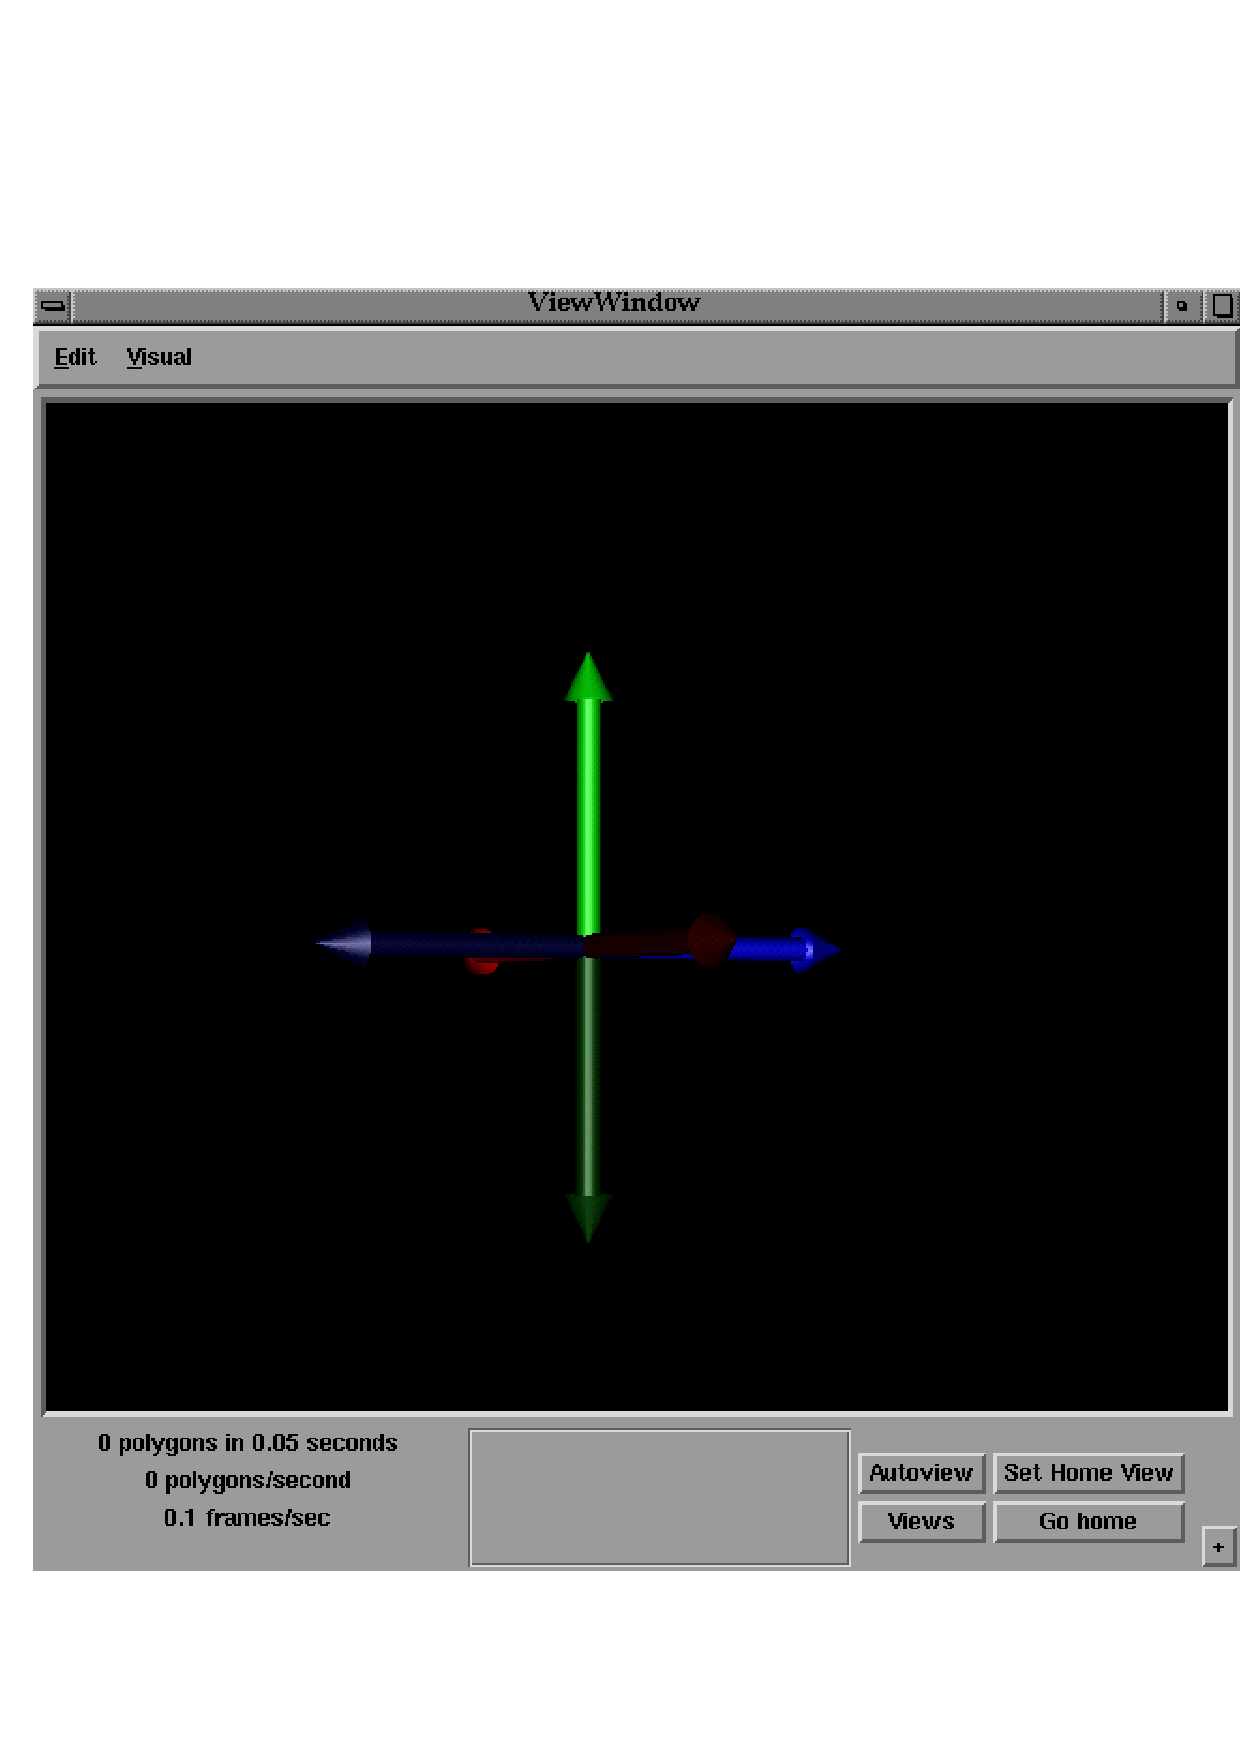
\epsfig{file=Figures/viewwindow.eps.gz,height=4in,
  bbllx=0, bblly=0, bburx=660, bbury=660}}}
%end{latexonly}
\begin{htmlonly}
  \newcommand{\viewerwindow}{%
  \htmladdimg[align=top,width=645,alt="module"]
  {../Figures/viewwindow.gif}}
\end{htmlonly}

%% View of the extended viewer window
%begin{latexonly}
  \newcommand{\extendedwindow}%
  {\centerline{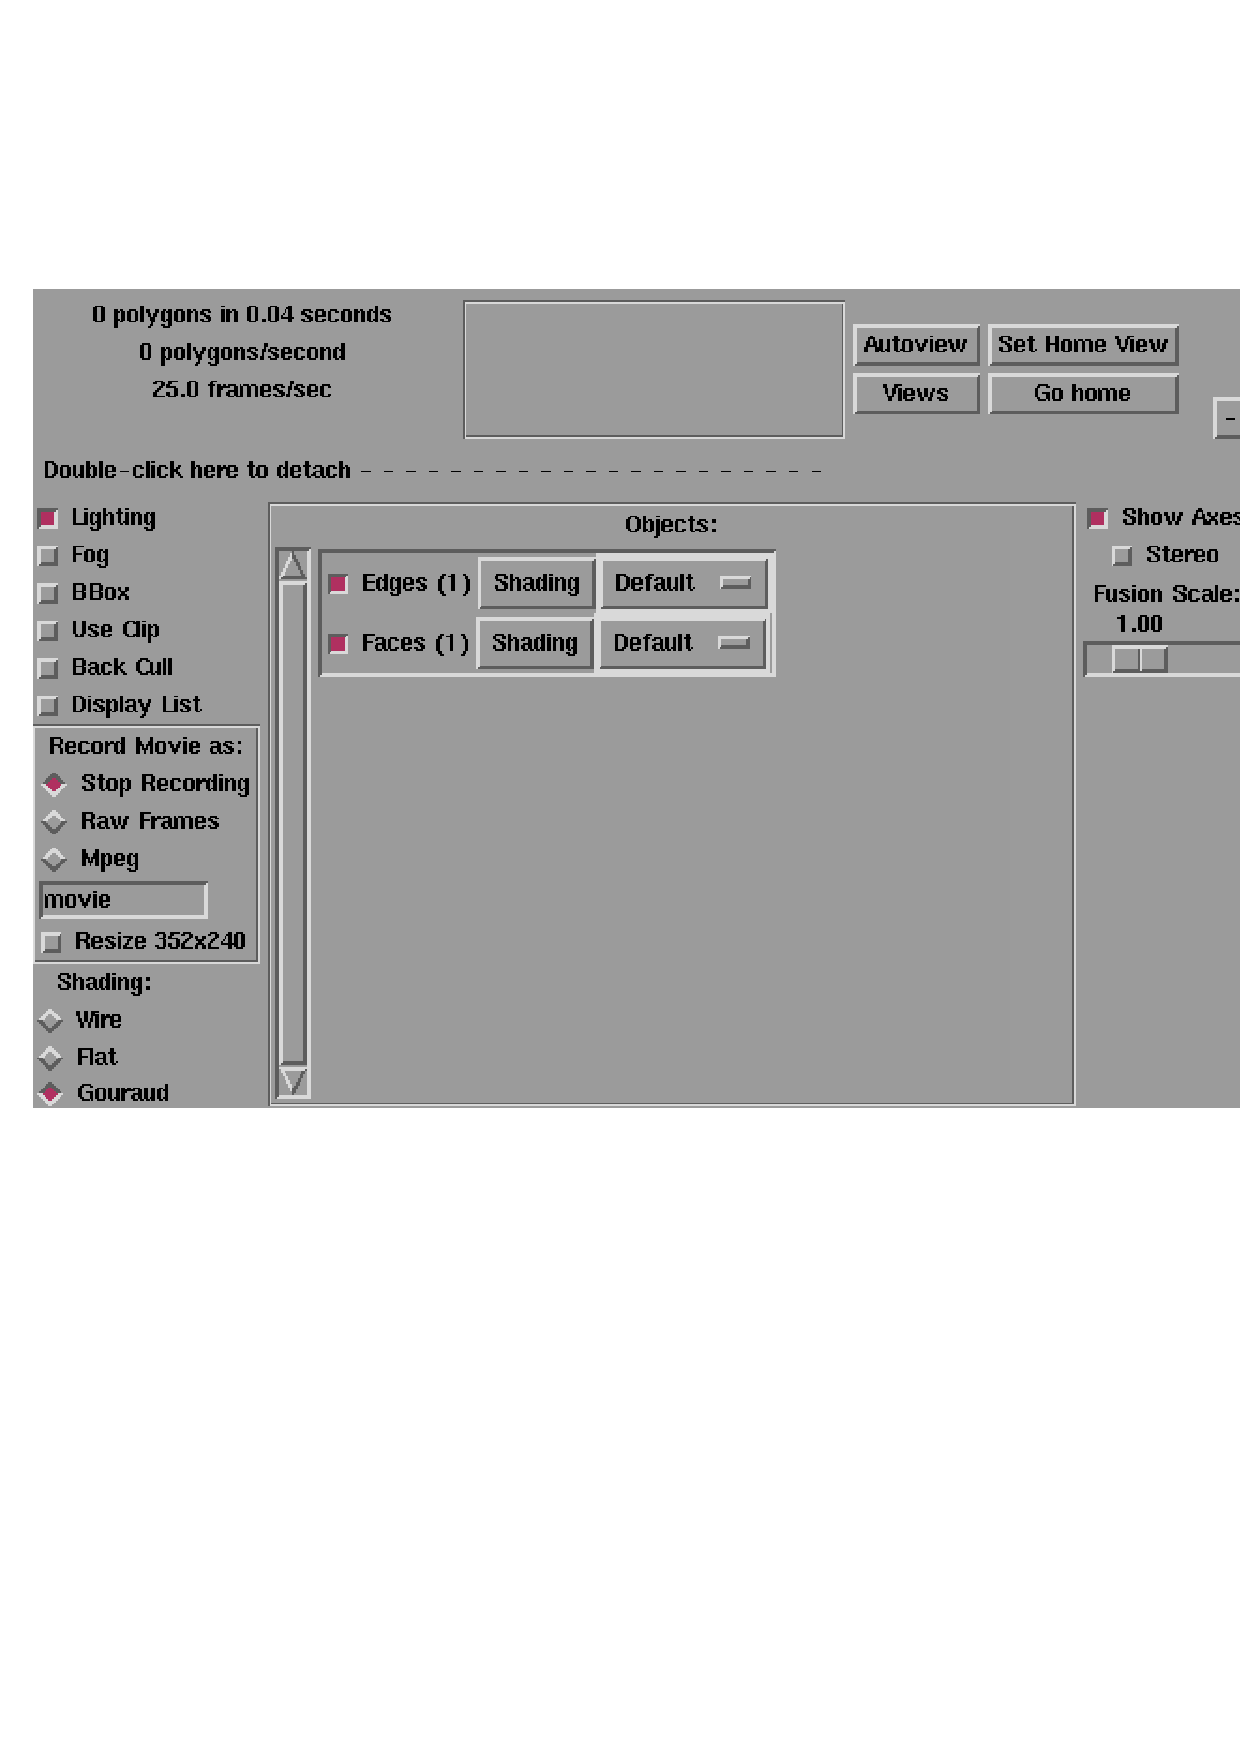
\epsfig{file=Figures/viewwindow-ext.eps.gz,height=4in,
  bbllx=16, bblly=310, bburx=600, bbury=703}}}
%end{latexonly}
\begin{htmlonly}
  \newcommand{\extendedwindow}{%
  \htmladdimg[align=top,width=649,alt="extended view window"]
  {../Figures/viewwindow-ext.jpg}}
\end{htmlonly}

%% Gauge widget image
%begin{latexonly}
  \newcommand{\gaugewidget}%
  {\centerline{\epsfig{file=Figures/widget-gauge.eps.gz,height=2in,
  bbllx=0, bblly=0, bburx=457, bbury=340}}}
%end{latexonly}
\begin{htmlonly}
  \newcommand{\gaugewidget}{%
  \htmladdimg[align=top,width=458,alt="gaugewidget"]
  {../Figures/widget-gauge.gif}}
\end{htmlonly}

%% Frame widget image
%begin{latexonly}
  \newcommand{\framewidget}%
  {\centerline{\epsfig{file=Figures/widget-frame.eps.gz,height=2in,
  bbllx=0, bblly=0, bburx=328, bbury=268}}}
%end{latexonly}
\begin{htmlonly}
  \newcommand{\framewidget}{%
  \htmladdimg[align=top,width=329,alt="framewidget"]
  {../Figures/widget-frame.gif}}
\end{htmlonly}

%% Box widget image
%begin{latexonly}
  \newcommand{\boxwidget}%
  {\centerline{\epsfig{file=Figures/widget-box.eps.gz,height=2in,
  bbllx=0, bblly=0, bburx=458, bbury=342}}}
%end{latexonly}
\begin{htmlonly}
  \newcommand{\boxwidget}{%
  \htmladdimg[align=top,width=459,alt="boxwidget"]
  {../Figures/widget-box.gif}}
\end{htmlonly}

%% Ring widget image
%begin{latexonly}
  \newcommand{\ringwidget}%
  {\centerline{\epsfig{file=Figures/widget-ring.eps.gz,height=2in,
  bbllx=0, bblly=0, bburx=507, bbury=467}}}
%end{latexonly}
\begin{htmlonly}
  \newcommand{\ringwidget}{%
  \htmladdimg[align=top,width=508,alt="ringwidget"]
  {../Figures/widget-ring.gif}}
\end{htmlonly}

%%%%%%%%%%%%%%%%%%%%%%%%%%%%%%%%%%%%%%%%%%%%%%%%%%%%%%%%%%%%%%%%%%%%%%
\newcommand{\graphics}{\emph{Graphics}}

\section{Visualization with the \viewer{}}
\label{sec:viewer}
\index{Viewer@\viewer{}}

This section describes the most frequently used \sr{} module,
the \viewer{}, which has the task of displaying interactive graphical
output to the computer screen.  You will use the \viewer{} any time you
wish to see a geometry, or spatial data.  More important for
computational steering (described in \secref{Computational
Steering}{sec:con-steering}) is that the \viewer{} provides access to
many simulation parameters and controls and thus indirectly initiates new
iterations of the simulation steps.

We begin with an overview of the \viewer{} window and its controls, then
describe in detail all the options and variations.

\subsection{Anatomy of the \viewer{} window}
\label{sec:viewer-anatomy} 
\index{Viewer@\viewer{}!anatomy}

The \viewer{} window contains two main areas, the upper portion,
called the \graphics{} window, which displays the graphics, and the
lower portion, where most of the control buttons are.
Figure~\ref{fig:viewwindow} contains an example of a \viewer{} window.
In the \graphics{} window, viewing is controlled mostly by means of the
mouse, mouse buttons, and various modifier keys (shift/control/alt).
In the lower window are a lot of buttons and sliders, the function of
which will become clear as you read this section of the manual.

\begin{figure}[htb]
  \begin{makeimage}
  \end{makeimage}
  \viewerwindow
%    \framebox{\parbox[3in]{\columnwidth}{The\dotfill Figure\\
%    \vspace{2in}\\
%    With some \dotfill dummy text}}
  \caption{\label{fig:viewwindow} The default \viewer{} window in \SR{}}
\end{figure}


First, try out the controls for the \graphics{} window by moving the mouse
to the center of the viewer window and clicking and holding the left button
and then dragging the mouse.  The objects should translate along with the
mouse.  Do the same operation with the middle mouse button and the objects
will rotate around a point in the center of the display.  The right mouse
button controls the scale of the display, zooming in when the mouse moves
downward or to the right.  See \secref{Mouse Control in the
Viewer}{sec:view-mouse} for details on using the mouse.

The controls visible along the bottom of the \viewer{} window set some basic
configurations as follows:
%
\begin{description}
\item [\button{Autoview}]\mbox{}
  
  Restores the display to a default condition. Very useful when some
  combination of settings results in the objects disappearing from the
  view window.

\item [\button{Set Home View}]\mbox{}
  
  Captures the setting of the current view so you can return to it
  later by clicking the Go home'' button.

\item [\button{Go home}]\mbox{}

  Restore the current home view.

\item [\button{Views}]\mbox{}
  
  Lists a number of standard viewing angles and orientations.  The
  view directions align with the Cartesian axes of the objects and the
  ``Up vector'' choice sets the orientation of the objects when viewed
  along the selected axis.

\end{description}

In the left corner of the control panel of the \viewer{} window are
performance indicators that document the current rendering speed for the
display.  The better the graphics performance of the workstation you
have, the higher the display rate.

You may reveal more controls by clicking the
\latexhtml{\fbox{+}}{\button{[+]}} button in the lower right corner of
the \viewer{} window.  The extended controls are described in
\secref{Extended control window} {sec:view-control}.


\subsubsection{Menus}
\index{Viewer@\viewer{}!menus}

At the top of the \viewer{} window are three pull-down menus.

\begin{description}
  \item [\menu{File}] \mbox{}

    Current contains only the \menuitem{Save image file...} item which
    allows you to save the contents of the \viewer{} window as an
    image to a file.

  \item [\menu{Edit}]\mbox{} 
    
    Provides access to controls for the background color for the
    window, as well as the clipping planes (requires the ``Use Clip''
    control to be selected in the extended controls described in
    \secref{Extended control window}{sec:view-control}).

  \item [\menu{Visual}]\mbox{}
    
    Allows you to select between different graphics hardware settings
    that are available on your workstation.  The list is ordered
    heuristically from most to least useful.

\end{description}

\subsection{Mouse Control in the \viewer{} Window}
\label{sec:view-mouse} 
\index{Viewer@\viewer{}!mouse controls}

The mouse controls within \SR{} are extensive and flexible.  The
resulting action depends on the choice of mouse button, any
simultaneously pressed control keys, and the way the mouse moves.  The
description in Tables~\ref{tab:view-mouse} and~\ref{tab:view-unicam}
below may seem overly complicated at first, but with a little playing,
it becomes intuitive (another way of saying you will learn it if you
use it enough).

\begin{table}[htb]
\begin{center}
  \begin{tabular}{|l|l|p{5in}|} \hline
    \multicolumn{3}{|c|}{\large Mouse Controls}\\ \hline \hline 
    \multicolumn{1}{|c|}{Control Key} & 
    \multicolumn{1}{|c|}{Button} & 
    \multicolumn{1}{|c|}{Action}\\ \hline
None & Left & Translate scene \\
     & Middle & \begin{raggedleft} Rotate scene about its center on an arc
    ball that surrounds it; rotation direction is a function of the
    initial mouse location so try different sites and note the
    response. \end{raggedleft}\\  
     & Right & Zoom or scale scene (downwards and to the right increases
     size, upwards or to the left decreases size) \\ \hline
Shift & Left & Select and move a widget in the display \\
      & Middle & Toggle through the modes for a widget \\
      & Right & Pop up a widget information window \\ \hline
Control & Left & Translate in the Z-direction, \ie{} zoom in and out of the
    screen (down moves closer, up further away).  Moving left and
    right increases the ``throttle'' of the Z-direction motion.  If
    the cursor is over a point on an object when clicked, this point
    becomes the center of the screen for translation.\\ 
      & Middle & Rotate the camera view about the eye point (using arcball
    motion). \\ 
      & Right & Unicam movement (see Table~\ref{tab:view-unicam})\\ \hline
\end{tabular}
\caption{\label{tab:view-mouse} Mouse controls for the \viewer{}}
\end{center}
\end{table}

\bigskip

\begin{table}
\begin{center}
\begin{tabular}{|l|l|p{3in}|} \hline
    \multicolumn{3}{|c|}{\large Unicam movement (Control key and right mouse
    button} \\ \hline \hline
    \multicolumn{1}{|c|}{Initial mouse location} & 
    \multicolumn{1}{|c|}{Action} & \\ 
    \hline
    Near edge of display & Rotate objects on the arc ball & \\
    Near the objects & Following behavior: & \\
    \hline
    & \multicolumn{1}{|c|}{Initial mouse movement} & 
    \multicolumn{1}{|c|}{Action}\\ \hline
    & Horizontal & Pan objects \\ 
    & Vertical & Zoom and pan: down = zoom in, up = zoom
    out, left and right= pan left and right) \\
    & None & Set rotation point for subsequent arc ball rotation.\\
    \hline
\end{tabular}
\caption{\label{tab:view-unicam} Autocam mouse controls in the \viewer{}}
\end{center}
\end{table}



\subsection{Extended Control Window}
\label{sec:view-control} 
\index{Viewer@\viewer{}!extended controls}

Click on the \button{[+]} button in the lower right corner of the
default \viewer{} window, and the window expands to reveal an extended
panel of control buttons, as shown in Figure~\ref{fig:extviewwindow}.
Click on the \button{[-]} sign that now replaces the \button{[+]} and
this extended panel disappears again.  Here we describe the control
options available in the extended control window.

\begin{figure}[htb]
  \begin{makeimage}
  \end{makeimage}
  \extendedwindow
%    \framebox{\parbox[3in]{\columnwidth}{The\dotfill Figure\\
%    \vspace{2in}\\
%    With some \dotfill dummy text}}
  \caption{\label{fig:extviewwindow} The lower portion of extended
    \viewer{} window in \SR{}} 
\end{figure}


\subsubsection{Object selector}

The lower portion of the extended \viewer{} window is divided into three
columns. The middle column contains a list of all the objects in the
display.  If the list becomes long enough, a scroll bar on the left
hand side controls which are visible.  For each entry in the list, we have
the following controls, reading from left to right:

\begin{itemize}
  \item At the left end of each of the
        objects in the list is a selection indicator that displays red
        when that object is 
        selected.  The \viewer{} window only displays those objects that
        are selected.
  \item Next comes the name of the object.
  \item The \button{Shading} control box that comes next determines the
        shading options that will be used for rendering the object.
        Options include: Lighting, BBox, Fog, Use Clip, Back Cull, and
        Display List (for descriptions, see
        \secref{Rendering controls}{sec:view-rendering}).
  \item At the right end of each entry is the lighting control, initially
        marked \menu{Default}.  In the Default setting, the common
        rendering controls described in \secref{Rendering
        controls}{sec:view-rendering} below apply.  Clicking this box
        reveals a set of options that will apply only to this object that
        include Wire, Flat and Gouraud.
\end{itemize}


\subsubsection{Rendering Controls}
\label{sec:view-rendering} 
\index{Viewer@\viewer{}!rendering}

The left column of the extended \viewer{} window contains controls that
apply to all of the selected objects with ``Default'' lighting selected.
Those without the Default setting will use their own, object specific
settings, as described in the previous section.  The lighting and shading
options available are:
%
\begin{description}
  \item [Lighting] Toggles whether or not the \viewer{} applies lighting
        to the display.  Objects without lighting have a constant
        color.
  \item [Fog] Draws objects with variable intensity based on their
        distance from the user, also known as ``depth cueing''.  Close
        objects appear brighter while more remote objects fade gradually
        into the background as a function of distance from the front.
  \item [BBox] Toggles whether the \viewer{} draws the selected objects
        in full detail or as a simple bounding box.
  \item [Use Clip] Applies up to six clipping planes to the display.
        To control the clipping plane locations, use the
        ``Edit -\ra{} Clipping Planes'' menu at the top of the
        \viewer{} window.
  \item [Back Cull] Displays only the forward facing facets of any surface
        objects in the display.
  \item [Display List] Cache the list of objects to be displayed; this
        option accelerates rendering when the content of the display does
        not change. 
  \item [Shading] Selects the type of shading for objects from the
        following options:
        \begin{description}
          \item [Wire] Show only the wire mesh of objects.
          \item [Flat] Draw each facet with a constant color.
          \item [Gouraud] Linearly interpolate the color across facets. 
        \end{description}
\end{description}

The right hand column of the extended \viewer{} window contains controls
for displaying the axes and creating stereoscopic rendering.  

\paragraph{Stereo viewing: } requires hardware LCD glasses synchronized
with the display so that visibility for each eye coincides with the
display of the appropriate view.  The ``Fusion Scale'' control provides a
means of setting the eye separation and thus setting the view that is most
suited to facial anatomy and distance from the screen.

\subsubsection{Making movies}
\label{sec:view-movies} 
\index{movies}

The \viewer{} window in \SR{} has simple controls for capturing sequences
of images into animations or movies.  Here we describe how this works.

In the left column of the extended \viewer{} window are controls for
selecting movie type and then initiating and stopping the acquisition of
individual frames in the movie.

\SR{} sends a frame to the movie after each ``redraw'' operation, \ie{}
each time anything moves in the display or any visualization parameter
changes.  If the MPEG package is available (See the
\htmladdnormallink{Installation Manual}{\installguideurl} for
details) then an option will be available for saving the animations as MPEG
movies.

There is also a button that forces the size of the graphical window to be
352x240 pixels in size, which is a standard format well suited to MPEG.

\subsection{Control widgets}
\label{sec:view-widgets} 

While the \hyperref{mouse controls}{mouse controls in
Section}{}{sec:view-mouse} describe many ways to interact with the contents
of the \viewer{}, SR{} also supports some powerful display widgets.
Examples of widgets capabilities include managing cutting surfaces colored
according to the local data values, displaying streamlines in vector
fields, or selecting sub-volumes within the display area for further
manipulation. 
 
We have tried to make interacting with these widgets as consistent as
possible so that, for example, controlling parameters is usually by clicking
and dragging on either a cylindrical ``collar'' or a sphere element of the
widget.  The original design of these modules was by James Purcifal
%%\cite{??}. 
Note that a single widget may have more than one purpose
depending on the context in which it exists.

In this section, we describe the widgets available within \SR{} and \BIOPSE{}.
The same widget may, for example, select a clipping or a display plane
through a three-dimensional object but may also set the seed points for a
streamline module.  

\subsubsection{Gauge Widget}
\label{sec:view-gaugewidget} 

\begin{figure}[htb]
  \begin{makeimage}
  \end{makeimage}
  \gaugewidget
%    \framebox{\parbox[3in]{\columnwidth}{The\dotfill Figure\\
%    \vspace{2in}\\
%    With some \dotfill dummy text}}
  \caption{\label{fig:gaugewidget} The gauge widget for setting location and
    density of seed points}
\end{figure}

\paragraph{Appearance: } The Gauge Widget consists of two spheres (A)
connected by a cylinder (B) with a small slider collar (C) on the cylinder.
There are also small resize cylinders extending from the spheres (D).

\paragraph{Purpose:} The primary use of the Gauge Widget is to set the
location and density of streamlines emerging from the long cylinder.  It
may also be used as a more general purpose three-dimensional slider or as a
source for a stream surface. 

\paragraph{Controls: } Clicking and dragging either sphere causes the
entire widget to move in space, rotating about the other sphere and
following along behind the selected sphere.  Dragging either of the resize
cylinders cases the size of the widget to change and dragging any point on
the main cylinder moves the whole widget without any change in orientation.
Dragging the slider collar changes the associated value, typically the
density of seed points for a streamline source.

\subsubsection{Frame Widget}
\label{sec:view-framewidget} 

\begin{figure}[htb]
  \begin{makeimage}
  \end{makeimage}
  \framewidget
%    \framebox{\parbox[3in]{\columnwidth}{The\dotfill Figure\\
%    \vspace{2in}\\
%    With some \dotfill dummy text}}
  \caption{\label{fig:framewidget} The frame widget for selecting
    cutting/projection planes}
\end{figure}


\paragraph{Appearance: } The Frame Widget consists of four cylinders
connected in a rectangle.  In the middle of each of the cylinders there is
a sphere (B), from which a resize cylinder extends (C).

\paragraph{Purpose:} The primary uses of the Frame Widget is for image
plane definition, for defining stream volumes, and as a "tie dye" as with
the Ring Widget described in \secref{Ring Widget}{sec:view-ringwidget}.

\paragraph{Controls: } Clicking and ragging a sphere on the widget will
cause the widget to rotate about it center; dragging on a resize cylinder
will move the associated edge and this extend or contract the rectangle.
Dragging any of the cylinder will drag the entire widget through space.


\subsubsection{Box Widget}
\label{sec:view-boxwidget} 

\begin{figure}[htb]
  \begin{makeimage}
  \end{makeimage}
  \boxwidget
%    \framebox{\parbox[3in]{\columnwidth}{The\dotfill Figure\\
%    \vspace{2in}\\
%    With some \dotfill dummy text}}
  \caption{\label{fig:boxwidget} The boxwidget for selecting sub-volumes}
\end{figure}

\paragraph{Appearance: } The Box Widget consists of twelve cylinders (A)
connected in a hexahedral box (three-dimensional rectangle) with cylinders
indicating on the edges of the box (B).  In the middle of each face of the
box is a sphere with a cylinder protruding from it (C) that provide resize
control.

\paragraph{Purpose:} The primary use of the Box Widget is to select a
subvolume of the workspace for further manipulation (\eg{} volume
rendering, isosurfaces, streamlines, mesh adaption) where the faces of the
widget act as orthogonal clipping planes.

\paragraph{Controls: } Clicking and dragging on one of the spheres rotates
the widget about its center without changing the position of the center.
Clicking on and dragging any resize handle
% What do these look like??
causes the associated face to extend without changing its orientation.
Dragging a cylinder causes the entire widget to move without changing its
orientation.

\subsubsection{Ring Widget}
\label{sec:view-ringwidget} 

\begin{figure}[htb]
  \begin{makeimage}
  \end{makeimage}
  \ringwidget
%    \framebox{\parbox[3in]{\columnwidth}{The\dotfill Figure\\
%    \vspace{2in}\\
%    With some \dotfill dummy text}}
  \caption{\label{fig:ringwidget} The ring widget for selecting
    cutting/projection planes}
\end{figure}


\paragraph{Appearance: } The Ring Widget consists of a ring (A) with four
embedded spheres (B), each with a resize cylindrical attached (D).  Between
two of the spheres is a sliding collar (C).  One of the resize cylinders
has a special material property (typically a different color from the other
cylinders) to indicate that it is the ``halfway point'' for the slider (E).

\paragraph{Purpose:} The primary use of the Ring Widget is to set the
density of streamlines emerging from the ring---the ring serves as a set of
seed points from which will emerge streamlines.  The Ring Widget can also
serve as a three-dimensional angle gauge, as a source for multiple
streamlines throughout its surface, as a source for a stream surface from
the outer ring, and as a source for a stream volume.  Another use is as a
color sheet, or ``tie dye'', in which the surface is colored as a function of
the scalar value of the field at each point.

\paragraph{Controls: } Clicking and dragging the slider collar along the
ring changes the density of the seed points or some other related
parameter.  Dragging the spheres controls the orientation of the Ring
Widget, while moving the resize cylinders changes the radius of the Ring
Widget about its center.  Dragging any other point on the ring moves the
ring in space without changing its radius or orientation.


%%% Local Variables: 
%%% mode: latex
%%% TeX-master: t
%%% End: 


\input{ui}

%%% Local Variables: 
%%% mode: latex
%%% TeX-master: "usersguide"
%%% End: 
